
\documentclass[aspectratio=169]{beamer}

\PassOptionsToPackage{hidelinks}{hyperref}
\usetheme[numbering=none]{metropolis}
\metroset{titleformat=regular}
\usepackage[english]{babel}
\usepackage[T1]{fontenc}
\usepackage[utf8]{inputenc}
\usepackage{amsmath, amssymb, mathtools}
\usepackage{microtype}
\usepackage{fourier}
\usepackage{xcolor}
\usepackage{mathpartir}
\usepackage{tikz}       % Core TikZ package
\usepackage{tikz-cd}    % For commutative diagrams
\usetikzlibrary{arrows.meta}   % For more arrow styles
\usetikzlibrary{matrix}        % For advanced matrix positioning
\usetikzlibrary{positioning}  % required for "below=of ..."

\setbeamercolor{normal text}{fg=black,bg=white}
\setbeamercolor{background canvas}{bg=white}
\setbeamercolor{structure}{fg=gray!60!black}
\setbeamercolor{title}{fg=gray!80!black}
\setbeamercolor{subtitle}{fg=gray!80!black}
\setbeamercolor{frametitle}{fg=white,bg=gray!70!black}
\setbeamercolor{section title}{fg=gray}
\setbeamercolor{progress bar}{fg=gray,bg=black!15}
\setbeamercolor{title separator}{fg=gray!70!black,bg=gray!70!black}
\metroset{block=transparent}
\setbeamertemplate{navigation symbols}{}
\metroset{
  progressbar=frametitle,
  numbering=fraction,
  titleformat frame=regular
}
\setbeamercolor{block title}{fg=white,bg=gray!70!black}
\setbeamercolor{block body}{fg=black,bg=gray!10}
\setbeamercolor{block title alerted}{fg=white,bg=gray!60!black}
\setbeamercolor{block body alerted}{fg=black,bg=gray!15}
\setbeamercolor{block title example}{fg=white,bg=gray!60!black}
\setbeamercolor{block body example}{fg=black,bg=gray!15}
\setbeamertemplate{blocks}[rounded][shadow=false]
\setbeamercolor{standout}{fg=white,bg=gray!70!black}
\setbeamercolor{palette primary}{fg=white,bg=gray!70!black}


\usepackage[cache=false]{minted}
\setminted{
  style=bw,
  fontsize=\footnotesize,
  breaklines=true,
  autogobble=true
}

\usepackage{pifont}

\newcommand{\checkedbox}{\fbox{\ding{51}}}
\newcommand{\crossedbox}{\fbox{\ding{55}}}


\title{Type Theory \& Categorical Models: A Unified Approach}
\subtitle{From Typelis to Logic to Closed Cartesian Categories}
\date{\today}
\author{Miguel Laredo Barbadillo}
\institute{Master's in Formal Methods in Computer Science}

\newcommand{\la}{\lambda}
\newcommand{\La}{\mathbf{\Lambda}}
\newcommand{\Ty}{\mathbf{T}}
\newcommand{\Tb}{\mathbf{B}}
\newcommand{\Bset}{\mathcal{B}}
\newcommand{\Vset}{\mathcal{V}}
\newcommand{\Tset}{\mathcal{T}}
\newcommand{\NAT}{\mathbb{N}}
\newcommand{\IF}{\texttt{IF}}
\newcommand{\SUCC}{\texttt{SUCC}}
\newcommand{\TRUE}{\texttt{TRUE}}
\newcommand{\FALSE}{\texttt{FALSE}}
\newcommand{\FST}{\texttt{FST}}
\newcommand{\SND}{\texttt{SND}}
\newcommand{\PAIR}{\texttt{PAIR}}
\newcommand{\NIL}{\texttt{NIL}}
\newcommand{\NOT}{\texttt{NOT}}
\newcommand{\AND}{\texttt{AND}}
\newcommand{\OR}{\texttt{OR}}
\newcommand{\cat}[1]{\mathbf{#1}}
\newcommand{\Hom}{\mathrm{Hom}}
\newcommand{\id}{\mathrm{id}}
\newcommand{\Ob}{\mathrm{Ob}}
\newcommand{\Mor}{\mathrm{Mor}}
\newcommand{\Set}{\cat{Set}}
\newcommand{\Top}{\cat{Top}}
\newcommand{\Grp}{\cat{Grp}}
\newcommand{\Fun}{\mathrm{Fun}}
\newcommand{\op}{^{\mathrm{op}}}
\newcommand{\lCalc}{$\la$-Calculus}
\newcommand{\lcalc}{$\la$-calculus}
\newcommand{\bred}{$\beta$-reduction}
\newcommand{\lterm}{$\la$-term}
\newcommand{\lterms}{$\la$-terms}
\newcommand{\lexpr}{$\la$-expression}
\newcommand{\aequiv}{$\alpha$-equivalence}
\newcommand{\aequivlt}{$\alpha$-equivalent}
\newcommand{\bequiv}{$\beta$-equivalence}
\newcommand{\functionfont}[1]{\mathbf{#1}}
\newcommand{\curly}{\mathrel{\leadsto}_\beta}

\newcommand{\betared}{\mathrel{\leadsto}_{\beta\eta}}
\newcommand{\betareds}{\mathrel{\leadsto}^*_{\beta\eta}}
\newcommand{\psred}{\mathrel{\rightrightarrows}}

\newcommand{\Sub}[1]{\functionfont{Sub}(#1)}
\newcommand{\Subb}{\functionfont{Sub}}
\newcommand{\FV}[1]{\functionfont{FV}(#1)}
\newcommand{\FVV}{\functionfont{FV}}
\newcommand{\orange}[1]{\textcolor{orange}{#1}}
\newcommand{\magenta}[1]{\textcolor{magenta}{#1}}
\newcommand{\blue}[1]{\textcolor{blue}{#1}}
\newcommand{\green}[1]{\textcolor{green}{#1}}
\newcommand{\myref}[1]{\textcolor{refcolor}{\hyperref[#1]{\ref*{#1}}}}
\newcommand{\subst}[2]{[#1 := #2]}
\newcommand{\step}{\curly}
\newcommand{\etaequiv}{$\eta$-equivalence}
\newcommand{\lam}[2]{\lambda #1.\,#2}
\newcommand{\app}[2]{#1.\,#2}
\newcommand{\abs}[2]{\la #1.\,#2}
\newcommand{\curlysym}{\mathrel{\leftrightarrow}_\beta}

\begin{document}

\maketitle

\section{Assumptions}

\begin{frame}{Assumptions}
  \textbf{Syntax of λ-terms}
  \begin{itemize}
  \item Variables, abstraction $\lambda x.\,M$, application $M\,N$
  \end{itemize}
  
  \textbf{Subterms \& Free variables}
  \begin{itemize}
  \item Subterm relation: $N \preceq M$ if $N$ occurs in $M$
  \item Free variables $\mathrm{FV}(M)$
  \item Combinators, when $\mathrm{FV}(M)=\varnothing$
  \end{itemize}
  
  \textbf{Substitution}
  \begin{itemize}
  \item Capture-avoiding substitution $M[x:=N]$
  \end{itemize}
\end{frame}


\begin{frame}
  \textbf{$\alpha$-equivalence}
  \begin{itemize}
  \item Renaming of bound variables: $\lambda x.M \equiv_\alpha \lambda y.\,M[x:=y]$ if $y\notin\mathrm{FV}(M)$
  \item Formal inference rules: reflexivity, congruence, renaming under binder
  \end{itemize}

  \textbf{$\beta$-reduction}
  \begin{itemize}
  \item Single-step: $(\lambda x.M) N \curly M[x:=N]$
  \item Multi-step: $\curly^{*}$ (reflexive, transitive closure)
  \item Redex = reducible expression; normal form = no redex
  \end{itemize}

  \textbf{$\eta$-equivalence}
  \begin{itemize}
  \item Extensionality: $\lambda x.\,M\,x =_\eta M$ if $x\notin\mathrm{FV}(M)$
  \end{itemize}
\end{frame}

\begin{frame}
  \textbf{Church--Rosser}
  \begin{itemize}
  \item Confluence of $\beta$-reduction:
    \[
      M \curly^{*} N_1 \text{ and } M \curly^{*} N_2 \text{ then } \exists P.\ N_1 \curly^{*} P \land N_2 \curly^{*} P
    \]
  \item Proof idea: parallel reduction / diamond property
  \end{itemize}

  \textbf{Normalization \& Examples}
  \begin{itemize}
  \item Strongly normalizing, weakly normalizing, non-normalizing
  \item $\lambda x.x$ (normal), $\Omega$ (non-normalizing), $(\lambda x.y)\,\Omega$ (reduces to $y$)
  \end{itemize}
\end{frame}

\begin{frame}
  \textbf{Encodings \& Fixed-points}
  \begin{itemize}
  \item Church numerals: $\mathrm{ZERO}, \mathrm{SUCC}, \mathrm{ADD}, \mathrm{MUL}, \mathrm{PRED}$
  \item Booleans: $\mathrm{TRUE}$, $\mathrm{FALSE}$, $\mathrm{IF}$
  \item Pairs: $\mathrm{PAIR}$, $\mathrm{FST}$, $\mathrm{SND}$
  \item Lists: $\mathrm{NIL}$, $\mathrm{CONS}$, $\mathrm{HEAD}$, $\mathrm{TAIL}$
  \item Fixed-point combinators: $Y, Z, \Theta$
  \end{itemize}
\end{frame}

\section{Typing}

\begin{frame}{Minimal Typing}
  \begin{block}{Types}
    \[
      \Tset ::= \Bset \mid \Tset \to \Tset
    \]

  \end{block}
  \[
    \lambda x : \sigma . x
    \vdash \lambda x : \sigma . x : \sigma \to \sigma
  \]
  \[
    \lambda x . x
    \vdash \lambda x . x : \sigma \to \sigma
  \]
  \vfill
  \hfill Church--Rosser \checkedbox \hfill Strongly Normalizing \checkedbox \hfill Weakly Normalizing \checkedbox \hfill
\end{frame}

\begin{frame}[fragile]{Type Extensions}
  \[
    \begin{aligned}
      \text{Product Types:} \quad & A \times B \to A &\qquad& A \times B \to B \\
      \text{Sum Types:}     \quad & A \to A + B &\qquad& B \to A + B
    \end{aligned}
  \]

  In terms of $\beta$-reduction they are all confluent.

  \begin{columns}[t]
    \column{0.35\textwidth}
    \begin{minted}[fontsize=\scriptsize]{Haskell}
      -- Product Type: A x B
      data Pair a b = Pair a b
      -- Projections
      pi1 :: Pair a b -> a
      pi1 (Pair x _) = x
      pi2 :: Pair a b -> b
      pi2 (Pair _ y) = y
    \end{minted}
    \column{0.35\textwidth}
    \begin{minted}[fontsize=\scriptsize]{Haskell}
      -- Sum type: A + B
      data Sum a b = InL a | InR b
      -- Injections
      inl :: a -> Sum a b
      inl = InL
      inr :: b -> Sum a b
      inr = InR
    \end{minted}
  \end{columns}
\end{frame}


\begin{frame}{Extended Typing -- Products}
  \begin{block}{Product Types}
    \[
      \Tset^\times ::= \Bset \mid \Tset^\times \to \Tset^\times \mid \Tset^\times \times \Tset^\times \mid 1
    \]
  \end{block}
  \begin{block}{Product Terms}
    \[
      \La^\times ::= x \mid \lambda x : \Tset.\ \La^\times \mid \La^\times \, \La^\times \mid \langle \La^\times, \La^\times \rangle \mid \pi_1 \La^\times \mid \pi_2 \La^\times \mid *
    \]
  \end{block}
\end{frame}

\begin{frame}{Extended Typing -- Sums}
  \begin{block}{Sum Types}
    \[
      \Tset^+ ::= \Bset \mid \Tset^+ \to \Tset^+ \mid \Tset^+ + \Tset^+ \mid 0
    \]
  \end{block}
  \begin{block}{Sum Terms}
    \[
      \La^+ ::= x 
      \mid \lambda x : \Tset.\ \La^+ 
      \mid \La^+\,\La^+ 
      \mid \iota_1 \La^+ 
      \mid \iota_2 \La^+ 
      \mid \mathsf{case}\; \La^+\; \mathsf{of}\;\iota_1 x \Rightarrow \La^+ \mid \iota_2 y \Rightarrow \La^+
      \mid \square_A\,\La^+
    \]
  \end{block}
\end{frame}

\begin{frame}{Extended Typing -- Products and Sums}
  \begin{block}{Product Sum Types}
    \[
      \Tset^{\times+} ::= \Bset 
      \mid \Tset^{\times+} \to \Tset^{\times+} 
      \mid \Tset^{\times+} \times \Tset^{\times+} 
      \mid \Tset^{\times+} + \Tset^{\times+} 
      \mid 1 
      \mid 0
    \]
  \end{block}
  \begin{block}{Product Sum Terms}
    \[
      \La^{\times+} ::= \La^\times \cup \La^+ 
    \]
  \end{block}
\end{frame}

\begin{frame}{Supplementary Material}
  \begin{itemize}
  \item \textbf{Church-Rosser Property (Untyped $\lambda$-Calculus)}:
    \begin{itemize}
    \item Confluence of reduction: if $M \curly^* N_1$ and $M \curly^* N_2$, there exists $P$ with $N_1 \curly^* P$ and $N_2 \curly^* P$
    \item Proven using \textbf{parallel $\beta\eta$-reduction}
    \end{itemize}
  \item \textbf{Weak Normalization (Typed $\lambda$-Calculus with Products)}:
    \begin{itemize}
    \item Every typable term eventually reduces to a normal form
    \item \textbf{Degree} is used as a measure of term complexity to structure the induction
    \item Extends standard normalization proofs to include \textbf{product types}
    \end{itemize}
  \end{itemize}
\end{frame}


\section{Curry Howard}
\begin{frame}{Intuitionistic Logic}
  \begin{itemize}
  \item Proofs must be \textbf{constructive}:  
    \begin{itemize}
    \item To prove $A \to B$, one must give a method that transforms any proof of $A$ into a proof of $B$.
    \item To prove $\exists x.\, P(x)$, one must provide a concrete witness $a$ together with a proof of $P(a)$.
    \end{itemize}

  \item \textbf{Excluded Middle} does not hold in general:  
    \(
    \not\vdash A \lor \neg A
    \)
    unless one can actually prove one of the disjuncts.

  \item Proofs by contradiction are not allowed.
  \end{itemize}
\end{frame}

\begin{frame}{The Isomorphism}
  \begin{table}[h!]
    \centering
    \begin{tabular}{|c|c|}
      \hline
      \textbf{Intuitionistic Logic} & \textbf{Typed $\lambda$-Calculus} \\
      \hline
      Proposition $A$ & Type $A$ \\
      Proof of $A$ & Term of type $A$ \\
      Implication $A \rightarrow B$ & Function type $A \to B$ \\
      Conjunction $A \land B$ & Product type $A \times B$ \\
      Disjunction $A \lor B$ & Sum type $A + B$ \\
      $\top$ & $1$ \\
      $\bot$ & $0$ \\
      Proof normalization & $\beta$-reduction \\
      \hline
    \end{tabular}
    \label{tab:curry-howard}
  \end{table}
\end{frame}

\begin{frame}{Example: Modus Ponens}
  \begin{block}{Modus Ponens}
    \[
      \inferrule*[right=\textsc{MP}]
      {P \to Q \quad P}
      {Q}
    \]
  \end{block}
  \[
    \begin{aligned}
      &(\lambda f : P \to Q.\, \lambda x : P.\, f\, x)\;\; f : P \to Q \;\; x : P 
      &&\vdash (P \to Q) \to P \to Q \\
      &\;\;\curly\;\;
        (\lambda x : P.\, f\, x) \;\; x : P 
      &&\vdash P \to Q \\
      &\;\;\curly\;\;
        f\, x 
      &&\vdash Q 
    \end{aligned}
  \]
\end{frame}


\section{Closed Cartesian Categories}

\begin{frame}{What is Category Theory}
  \begin{itemize}
  \item Category theory is a general theory of mathematical structures and their relations

  \item The focus of study are relations among objects, and not the objects themselves
  \end{itemize}
\end{frame}

\begin{frame}{Definition of Category}
  \begin{block}{Category}
    A \textbf{category} $\mathcal{C}$ consists of:
    \begin{itemize}
    \item A collection of \textbf{objects}: $\mathrm{Ob}(\mathcal{C})$
    \item For each pair of objects $A, B \in \mathrm{Ob}(\mathcal{C})$,
      a set of arrows $\mathrm{Hom}_{\mathcal{C}}(A,B)$
    \item For each $A \in \mathrm{Ob}(\mathcal{C})$, an \textbf{identity morphism}  
      $\mathrm{id}_A \in \mathrm{Hom}_{\mathcal{C}}(A,A)$
    \item For each $f \in \mathrm{Hom}_{\mathcal{C}}(A,B)$ and  
      $g \in \mathrm{Hom}_{\mathcal{C}}(B,C)$, a \textbf{composition}  
      $g \circ f \in \mathrm{Hom}_{\mathcal{C}}(A,C)$
    \end{itemize}
  \end{block}
  \begin{block}{Axioms}
    These must satisfy:
    \begin{itemize}
    \item \textbf{Associativity:} $(h \circ g) \circ f = h \circ (g \circ f)$.
    \item \textbf{Identity:} $\mathrm{id}_B \circ f = f = f \circ \mathrm{id}_A$.
    \end{itemize}
  \end{block}
\end{frame}

\begin{frame}[fragile]{Example: Preorder as a Category}
  \[
    \begin{tikzcd}[row sep=2cm, column sep=2cm]
      a \arrow[r, "f"] \arrow[rr, bend left=50, "g \circ f"] \arrow[rrr, bend left=75, "(h \circ g) \circ f = h \circ (g \circ f) = h \circ g \circ f "] & b \arrow[r, "g"] \arrow[rr, bend right=50, "h \circ g"] & c \arrow[r, "h"] & d \\
    \end{tikzcd}
  \]
\end{frame}

\begin{frame}[fragile]{Example: Preorder as a Category}
  \[
    \begin{tikzcd}[row sep=2cm, column sep=2cm]
      a \arrow[r, "\leq"] \arrow[rr, bend left=50, "\leq"] \arrow[rrr, bend left=75, "\leq"] & b \arrow[r, "\leq"] \arrow[rr, bend right=50, "\leq"] & c \arrow[r, "\leq"] & d \\
    \end{tikzcd}
  \]
\end{frame}

\begin{frame}[fragile]{Commutative Diagrams}
  \begin{block}{Definition}
    A diagram in a category \(\mathcal{C}\) is said to \textbf{commute} if, for any two objects connected by more than one path of morphisms, all paths compose to the same morphism.
  \end{block}
  \[
    \begin{tikzcd}
      A \arrow[r, "f"] \arrow[rd, "h"'] & B \arrow[d, "g"] \\
      & C
    \end{tikzcd}
  \]
  This triangle commutes if:
  \[
    g \circ f = h
  \]
  meaning the two ways of going from \(A\) to \(C\) are equal. Commutativity ensures consistency of compositions.
\end{frame}

\begin{frame}[fragile]{Injectivity via Arrows}
  \begin{block}{Injective Function}
    A function $f : X \to Y$ is \textbf{injective} if
    \(
    \forall x_1, x_2 \in X, f(x_1) = f(x_2) \implies x_1 = x_2
    \)
  \end{block}
  \begin{block}{Monomorphism}
    A morphism $f : X \to Y$ in a category $\mathcal{C}$ is a \textbf{monomorphism} if for all objects $Z$ and morphisms $g_1, g_2 : Z \to X$,
    \[
      f \circ g_1 = f \circ g_2 \implies g_1 = g_2.
    \]
    \begin{itemize}
    \item In the category \textbf{Set}, monomorphisms coincide with injective functions.
    \item This definition generalizes injectivity to arbitrary categories.
    \end{itemize}
  \end{block}
\end{frame}

\begin{frame}[fragile]{Universal Constructions}
  \begin{block}{Definition}
    Universal Constructions are a way of defining properties up to Isomorphism using only arrows
  \end{block}
\end{frame}

\begin{frame}[fragile]{Example of Universal Construction: Terminal Object}
  \begin{block}{Definition}
    An object \(T\) in a category \(\mathcal{C}\) is \emph{terminal} if for every object \(X\in\operatorname{Ob}(\mathcal{C})\) there exists a unique morphism
    \[
      !_X: X \longrightarrow T
    \]
  \end{block}
  Take terminal objects $A, B \in \operatorname{Ob}(\mathcal{C})$. Then,
  \begin{center}
    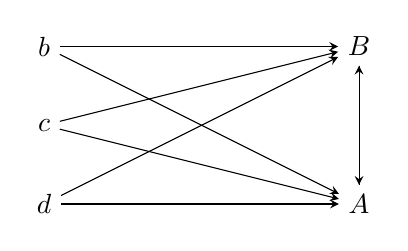
\begin{tikzpicture}[>=stealth, node distance=2cm]
      \node (A1) at (0,2) {$b$};
      \node (A2) at (0,1) {$c$};
      \node (A3) at (0,0) {$d$};

      \node (A0) at (4,0) {$A$};
      \node (B0) at (4,2) {$B$};

      \draw[->] (A1) -- (A0);
      \draw[->] (A2) -- (A0);
      \draw[->] (A3) -- (A0);

      \draw[->] (A1) -- (B0);
      \draw[->] (A2) -- (B0);
      \draw[->] (A3) -- (B0);

      \draw[->] (A0) -- (B0);
      \draw[->] (B0) -- (A0);
    \end{tikzpicture}
  \end{center}
  \[
    A \cong B
  \]
\end{frame}

\begin{frame}[fragile]{Products}
  \[
    \begin{tikzcd}[row sep=huge, column sep=huge]
      &  & \\
      A & A \times B  \arrow[l, "\pi_1"] \arrow[r, "\pi_2"'] & B
    \end{tikzcd}
  \]

  \[
    A = \big\{2, 4, 6\big\} \quad B = \big\{3, 6, 9\big\} \quad A \times B = \big\{(2, 3), (2, 6), (2, 9), (4, 3), \dots\big\}
  \]
  
\end{frame}

\begin{frame}[fragile]{Products}
  \[
    \begin{tikzcd}[row sep=huge, column sep=huge]
      & X \arrow[dl, "f"'] \arrow[dr, "g"] & \\
      A & A \times B  \arrow[l, "\pi_1"] \arrow[r, "\pi_2"'] & B
    \end{tikzcd}
  \]
  \[
    A = \big\{2, 4, 6\big\} \quad B = \big\{3, 6, 9\big\} \quad A \times B = \big\{(2, 3), (2, 6), (2, 9), (4, 3), \dots\big\}
  \]
  \[
    X = \big\{ 1, 2, 3 \big\} \quad f(x) = 2x \quad g(x) = 3x
  \]
\end{frame}

\begin{frame}[fragile]{Products}
  \[
    \begin{tikzcd}[row sep=huge, column sep=huge]
      & X \arrow[dl, "f"'] \arrow[dr, "g"] \arrow[d, dashrightarrow, "{\langle f,g \rangle}"] & \\
      A & A \times B \arrow[l, "\pi_1"] \arrow[r, "\pi_2"'] & B
    \end{tikzcd}
  \]
  \[
    A = \big\{2, 4, 6\big\} \quad B = \big\{3, 6, 9\big\} \quad A \times B = \big\{(2, 3), (2, 6), (2, 9), (4, 3), \dots\big\}
  \]
  \[
    X = \big\{ 1, 2, 3 \big\} \quad f(x) = 2x \quad g(x) = 3x
  \]
  \[
    \langle f, g \rangle = \langle 2x, 3x \rangle
  \]
\end{frame}

\begin{frame}[fragile]{Products}
  \begin{block}{Definition: Product}
  \[
    \begin{tikzcd}[row sep=huge, column sep=huge]
      & X \arrow[dl, "f"'] \arrow[dr, "g"] \arrow[d, dashrightarrow, "{\langle f,g \rangle}"] & \\
      A & { P } \arrow[l, "\pi_1"] \arrow[r, "\pi_2"'] & B
    \end{tikzcd}
  \]
  \end{block}
\end{frame}

\begin{frame}{Duality in Category Theory}
  \textbf{Definition:}  
  For any category \(\mathcal{C}\), the \textbf{dual category} \(\mathcal{C}^{\mathrm{op}}\) is defined by:
  \begin{itemize}
    \item \(\mathrm{Ob}(\mathcal{C}^{\mathrm{op}}) = \mathrm{Ob}(\mathcal{C})\)
    \item \(\mathrm{Hom}_{\mathcal{C}^{\mathrm{op}}}(A,B) = \mathrm{Hom}_{\mathcal{C}}(B,A)\)
    \item Composition in \(\mathcal{C}^{\mathrm{op}}\) is reversed: if \(f: B \to C\) and \(g: A \to B\) in \(\mathcal{C}\), then \(g \circ f\) in \(\mathcal{C}^{\mathrm{op}}\) corresponds to \(f \circ g\)
  \end{itemize}

  \vspace{0.5em}
  \textbf{Intuition:} Flip all arrows in the category.
\end{frame}

\begin{frame}[fragile]{Example: Duality of Products -- Coproducts}
  \[
    \begin{tikzcd}[row sep=huge, column sep=huge]
      & X \arrow[dl, "f"'] \arrow[dr, "g"] \arrow[d, dashrightarrow, "{\langle f,g \rangle}"] & \\
      A & { A \times B } \arrow[l, "\pi_1"] \arrow[r, "\pi_2"'] & B
    \end{tikzcd}
    \quad \Rightarrow \quad
    \begin{tikzcd}[row sep=huge, column sep=huge]
      A \arrow[r, "\iota_1"] \arrow[dr, "f"'] & A + B \arrow[d, dashrightarrow, "{[f,g]}"] & B \arrow[l, "\iota_2"'] \arrow[dl, "g"] \\
      & X &
    \end{tikzcd}
  \]
\end{frame}

\begin{frame}[fragile]{Exponential Object}
  \begin{block}{Definition: Exponential}
  \[
    \begin{tikzcd}[row sep=huge, column sep=huge]
      C \times A \ar[rr, dashed, "\lambda f \times 1_A"] \ar[dr, "f"'] & & B^{A} \times A \ar[dl, "\mathrm{ev}_{A,B}"] \\
      & B &
    \end{tikzcd}
  \]
  \end{block}
  \begin{columns}
    \column{0.55\textwidth}
    \begin{itemize}
      \item $f : C \times A \to B$ \hfill (uncurried)
      \item $\lambda f : C \to B^A$ \hfill (curried)
      \item $\mathrm{ev}_{A,B} : B^A \times A \to B$ \hfill (evaluation)
    \end{itemize}
    \column{0.45\textwidth}
    \[
      f = \lambda (c,a).\, g(c,a)
    \]
    \[
      \lambda f = \lambda c.\, (\lambda a.\, g(c,a))
    \]
    \[
      f = \mathrm{ev}_{A,B} \circ ((\lambda f) \times \id_A)
    \] 
  \end{columns}

\[
  f = \lambda (a,b).\, g(a,b)
  \quad\leadsto\quad
  \lambda f = \lambda a.\,\lambda b.\, g(a,b)
\]
\end{frame}




\begin{frame}[fragile]{Cartesian Closed Category}
  \begin{block}{Definition: Closed Cartesian Category}
  A category \(\mathcal{C}\) is \textbf{cartesian closed} if:  
  \begin{itemize}
    \item \(\mathcal{C}\) has a \underline{\textbf{terminal object} \(1\)}
    \item \(\mathcal{C}\) has \textbf{binary products} \underline{\(A \times B\) for all objects \(A, B\)}
    \item \(\mathcal{C}\) has \textbf{exponentials}: \underline{for all objects \(A, B\), there exists \(B^A\)} such that
    \[
      \mathrm{Hom}_{\mathcal{C}}(X \times A, B) \cong \mathrm{Hom}_{\mathcal{C}}(X, B^A)
    \]
    naturally in \(X\)
  \end{itemize}
  \end{block}

  \vspace{0.5em}
  \textbf{Intuition:} Functions as objects — “product + exponent = function space.”
\end{frame}

\begin{frame}{The Lambek Extension}

\begin{table}[h!]
  \centering
  \label{tab:CHL}
  \begin{tabular}{|c|c|c|}
    \hline
    \textbf{Intuitionistic Logic} & \textbf{Typed $\lambda$-Calculus} & \textbf{Category Theory / Lambek} \\
    \hline
    Proposition $A$ & Type $A$ & Object $A$ \\
    Proof of $A$ & Term of type $A$ & Morphism $f: 1 \to A$ \\
    Implication $A \rightarrow B$ & Function type $A \to B$ & Exponential object $B^A$ \\
    Conjunction $A \land B$ & Product type $A \times B$ & Product $A \times B$ \\
    $\top$ & $1$ & Terminal object $1$ \\
    Proof normalization & $\beta$-reduction & { Commutativity of diagrams } \\
    \hline
  \end{tabular}
  \label{tab:curry-howard-lambek}
\end{table}

\begin{table}[h!]
  \centering
  \label{tab:CHL-sum}
  \begin{tabular}{|c|c|c|}
    \hline
    \textbf{Intuitionistic Logic} & \textbf{Typed $\lambda$-Calculus} & \textbf{Category Theory / Lambek} \\
    \hline
    Disjunction $A \lor B$ & Sum type $A + B$ & Coproduct $A + B$ \\
    $\bot$ & Empty type $0$ & Initial object $0$ \\
    \hline
  \end{tabular}
\end{table}
  
\end{frame}



\begin{frame}[fragile]{Perspectives}
  \begin{center}
      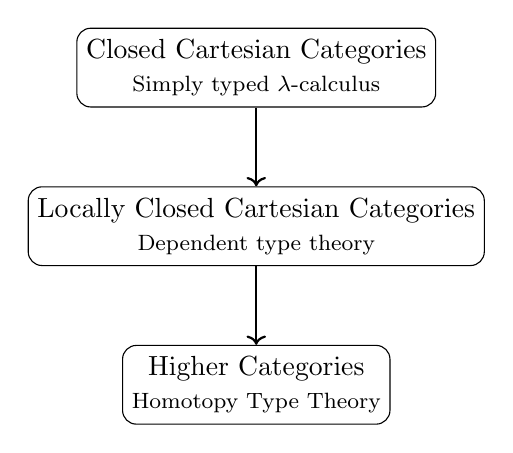
\begin{tikzpicture}[node distance=1cm, every node/.style={draw, rounded corners=5pt, minimum width=3cm, minimum height=1cm, align=center}]
        \node (ccc) {Closed Cartesian Categories \\ \footnotesize Simply typed $\lambda$-calculus};
        \node (lccc) [below=of ccc] {Locally Closed Cartesian Categories \\ \footnotesize Dependent type theory};
        \node (higher) [below=of lccc] {Higher Categories \\ \footnotesize Homotopy Type Theory};
        \draw[->, thick] (ccc) -- (lccc);
        \draw[->, thick] (lccc) -- (higher);
      \end{tikzpicture}
  \end{center}
\end{frame}


\begin{frame}{Errata}
  p.31 (Adgda -> Agda)
  
  p.31 (Duplicated definition + Empty definition)

  p.38 (Ax -> Assume-X)

  p.48 (belements -> elements)

  p. (Locally Cartesian Closed -> Locally Closed Cartesian)
  
  Inconsistencies here and there + Formatting issues
\end{frame}

\begin{frame}[standout]
  \textbf{\Huge{Q\&A.}}
\end{frame}

\end{document}



